\documentclass{beamer}
\usepackage[utf8]{inputenc}
\usepackage{polski}
\usepackage[polish]{babel}
\usepackage[T1]{fontenc}
\usepackage{multicol}

\mode<presentation>
{
  \usetheme{Madrid}
  \usecolortheme{beaver}
  \usefonttheme{default}
  \setbeamertemplate{navigation symbols}{}
  \setbeamertemplate{caption}[numbered]
} 


\usepackage{graphicx}
\DeclareGraphicsExtensions{.png,.jpg}

\title[Hadoop]{Hadoop}
\author{Jakub Podeszwik}
\institute{infoShare Academy}
\date{20.03.2019}

\AtBeginSection[]{
	\begin{frame}
		\begin{center}
			\usebeamerfont{section title}\Large\insertsection
		\end{center}
	\end{frame}
}

\begin{document}

\begin{frame}
  \titlepage
\end{frame}

\begin{frame}{Warsztat}
	\begin{itemize}
		\item 2 dni
		\item 10\% prezentacja
		\item 40\% live coding
		\item 50\% zadań głównie programistycznych
	\end{itemize}
\end{frame}

\begin{frame}{Hadoop}
	\begin{figure}
		
\includegraphics[width=\textwidth,height=7cm,keepaspectratio=true]{hadoop}
	\end{figure}
\end{frame}
\begin{frame}{HDFS}
	\begin{figure}
		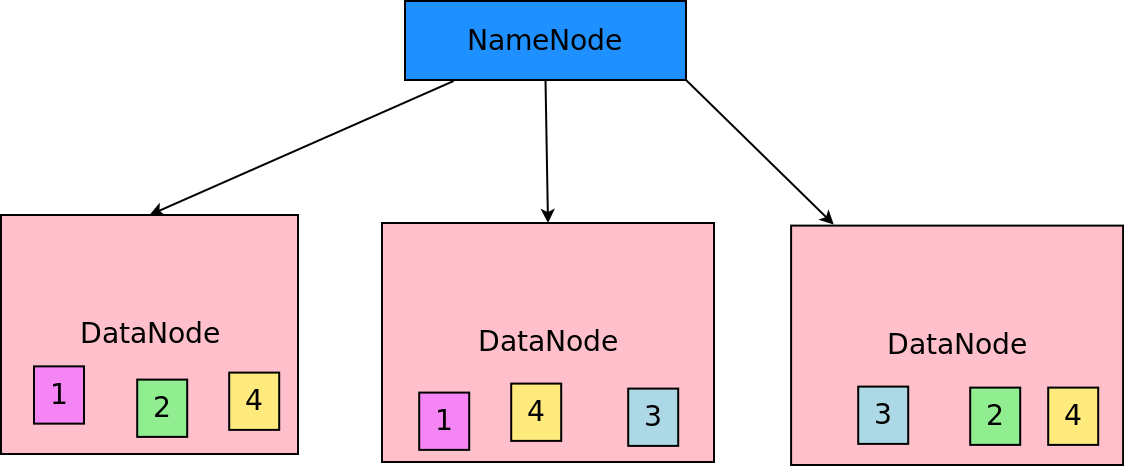
\includegraphics[width=\textwidth,height=7cm,keepaspectratio=true]{hdfs}
	\end{figure}
\end{frame}
\begin{frame}{YARN}
	\begin{figure}
		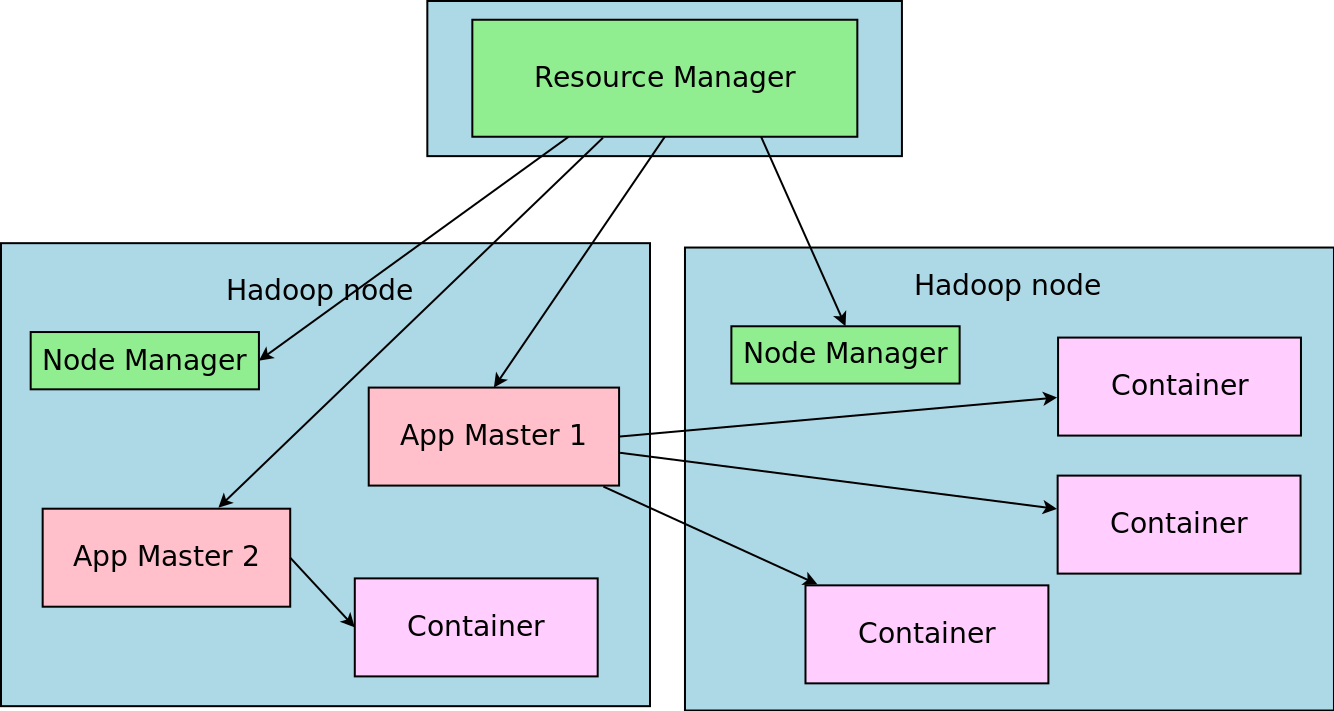
\includegraphics[width=\textwidth,height=7cm,keepaspectratio=true]{yarn}
	\end{figure}
\end{frame}
\begin{frame}{MapReduce}
	\begin{figure}
		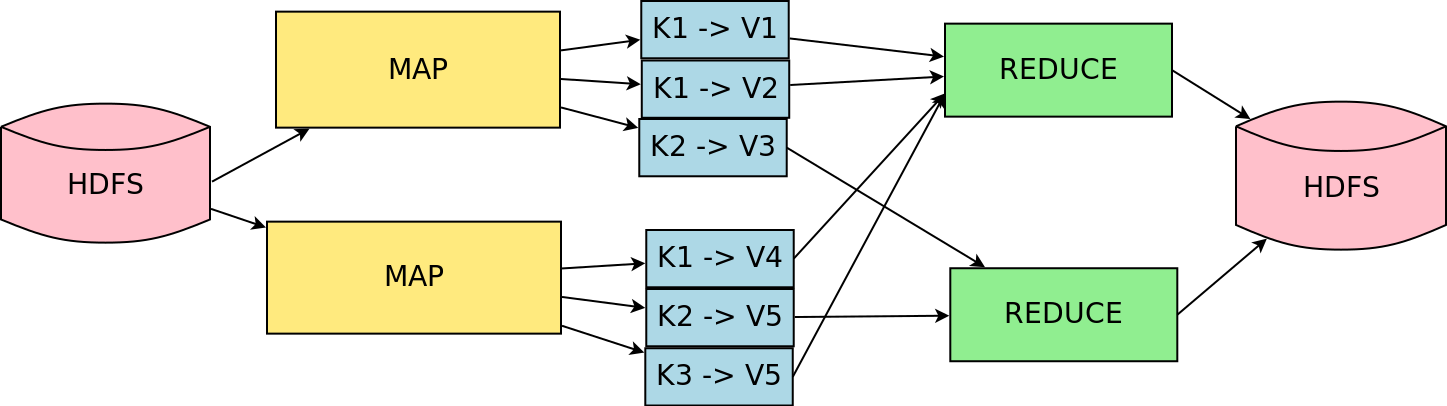
\includegraphics[width=\textwidth,height=7cm,keepaspectratio=true]{mapreduce}
	\end{figure}
\end{frame}
\begin{frame}{Hive}
	\begin{figure}
		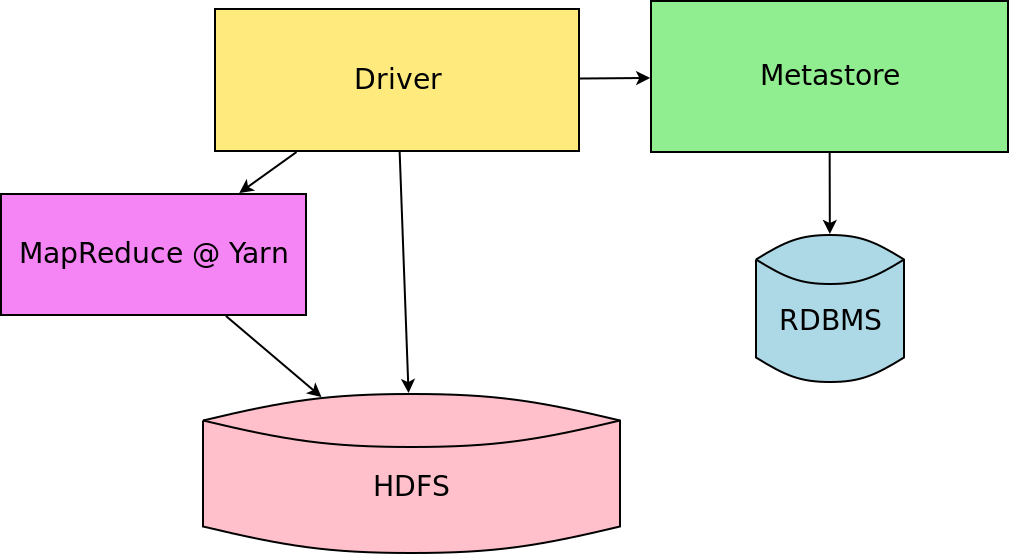
\includegraphics[width=\textwidth,height=7cm,keepaspectratio=true]{hive}
	\end{figure}
\end{frame}
\begin{frame}{Sqoop}
	\begin{figure}
		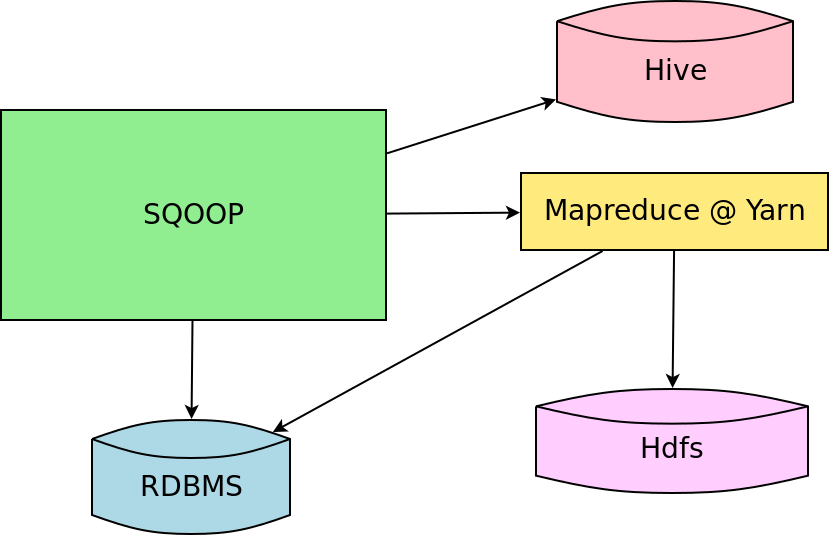
\includegraphics[width=\textwidth,height=7cm,keepaspectratio=true]{sqoop}
	\end{figure}
\end{frame}
\begin{frame}{Flume}
	\begin{figure}
		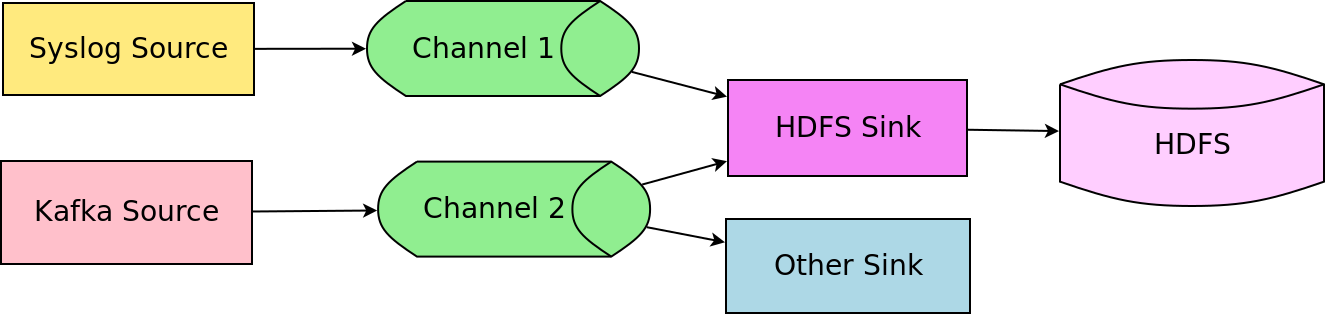
\includegraphics[width=\textwidth,height=7cm,keepaspectratio=true]{flume}
	\end{figure}
\end{frame}
\begin{frame}{Oozie}
	\begin{figure}
		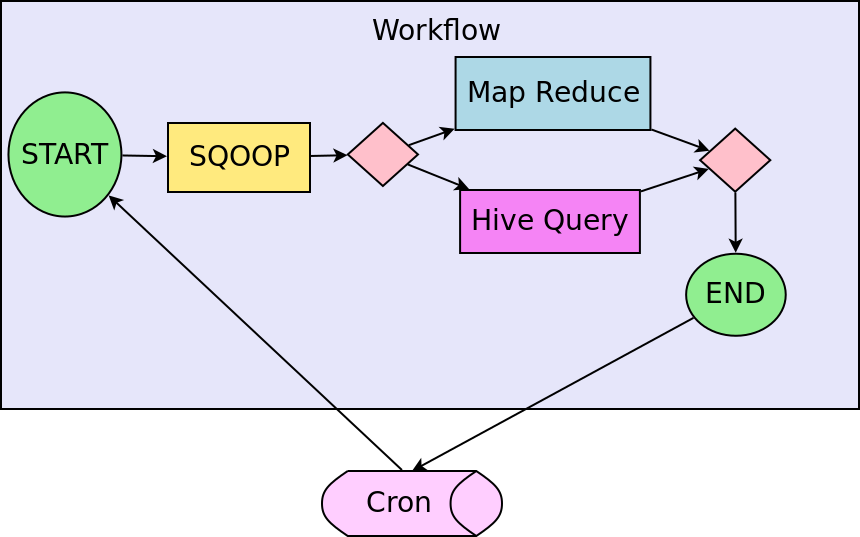
\includegraphics[width=\textwidth,height=7cm,keepaspectratio=true]{oozie}
	\end{figure}
\end{frame}
\begin{frame}{Hue}
	\begin{figure}
		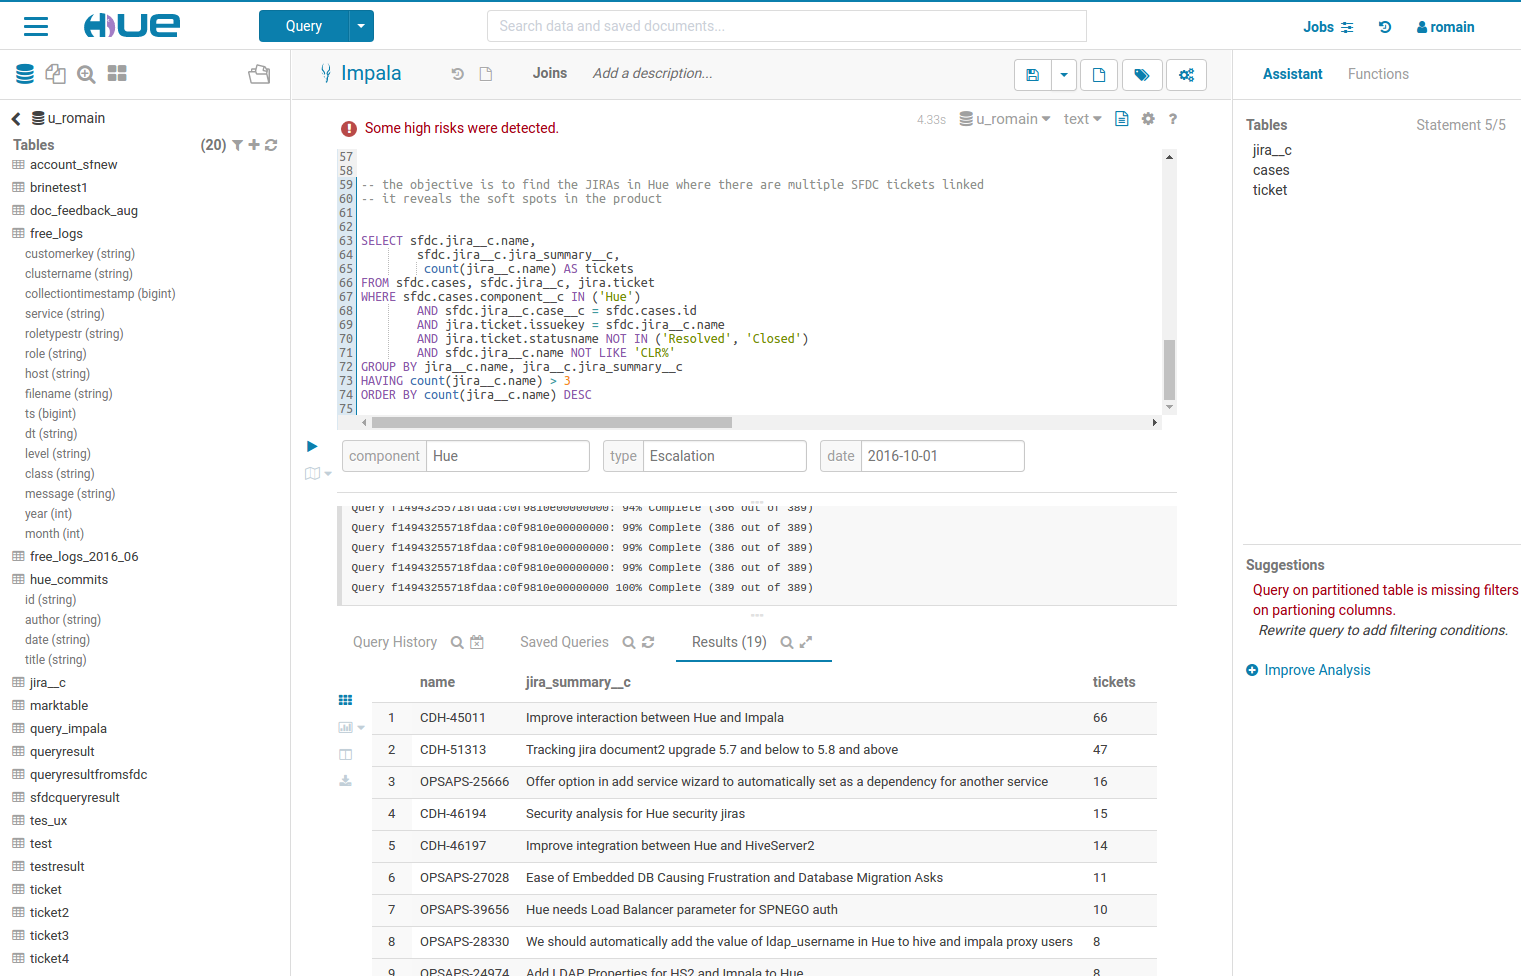
\includegraphics[width=\textwidth,height=7cm,keepaspectratio=true]{hue}
	\end{figure}
	\begin{center}
		{\tiny (http://gethue.com/)}
	\end{center}
\end{frame}
\begin{frame}{Dystrybucje}
	\begin{multicols}{2}
		\begin{figure}
			
\includegraphics[width=5cm,height=4cm,keepaspectratio=true]{distributions/mapr}
			
\includegraphics[width=5cm,height=4cm,keepaspectratio=true]{distributions/hortonworks}
		\end{figure}
	\end{multicols}
	\begin{figure}
		
\includegraphics[width=5cm,height=4cm,keepaspectratio=true]{distributions/cloudera}
	\end{figure}
\end{frame}


\begin{frame}{Dzień 1}
	\begin{enumerate}
		\item HDFS
		\item MapReduce
		\item Hadoop Streaming
		\item Sqoop
	\end{enumerate}
\end{frame}
\begin{frame}{Dzień 2}
	\begin{enumerate}
		\item Flume
		\item Hive
		\item Hive UDFs
		\item Oozie
	\end{enumerate}
\end{frame}

\section{Pytania?}

\end{document}
